\chapter{Demo program} \label{chap:results}

We present a simple test program to demonstrate the functions and capabilities of Lvis library. To do so, we've used Mitsuba, a physically based renderer developed by Wenzel Jakob. Apart from LuxRenderer, it's the only one of the larger open source renderers which supports Metropolis Light Transport. The downside is that Mitsubas plugin oriented program structure (described below) makes the usage of our library (which requires access to light paths and their vertex data) rather complicated and impractical. Instead, we opted to use it separately, utilizing it's path space MLT algorithm together with its built-in path print function to generate a mass of light paths, which we then stored in a text file and later parsed into our demonstration program. This, of course, prevents us from showing the feature of selected path feedback, but with the rest of the visualisation qualities unaffected - and probably even a minor speed up in gathering of each new light path - that's just a minor setback. 

\section{Mitsuba data structure and path generation}

For the purposes of our demonstration, the only segments of code from the Mitsuba sources we were interested in were the ones regarding the light path structure. With the core functionality split between four libraries - one of which (\texttt{libbidir}) was containing the support framework for all bidirectional path tracing algorithms - it was straightforward to locate the data structures of Mitsubas internal path format. Additionally, this class already had a method of printing it's data into a single \texttt{std::string}.

Next, we needed to find the MLT mutation and rendering cycle, from which these paths are instantiated and mutated. All rendering algorithms in Mitsuba are handled as integrator plugins - the plugin part meaning that they are loaded and compiled on demand at runtime, and the integrator moniker implying that at heart, these algorithms perform integration over a high-dimensional space. Each of these integrators contain a \emph{work unit}, which performs all of the heavy lifting and also allows for parallelization, with multiple work units each solving a different subset of the integral. Therefore, the only file we've needed to modify was \texttt{mlt\_proc.cpp}, containing the worker unit class for the MLT algorithm. 

Our changes were fairly minimal, only adding an output \texttt{filestream}, which we then supplied with the output of \texttt{print} function of the \texttt{current} path pointer. Our program is able to correctly read and parse any textfile consisting of data aggregated using this function. Note that we're visualizing only the \emph{accepted} light paths, and rejection of the proposed mutation means that subsequent light paths will be identical. This is not viewed as a problem, since it keeps a record of rejections in our visualisation (without the need to parse all of the proposed paths). Since we've only used core c++ functionality in our modifications, there was no need to tamper with the \texttt{.cmake} configuration. Apart from the light path data, Mitsuba also provides us with a nice set of statistics from the rendering(\ref{lst:mlt-res} - we have omitted the information on texturing since it's not relevant to this work).

\begin{listing}
\begin{minted}[mathescape,
               numbersep=5pt,
               frame=lines,
               framesep=2mm]{xml}
* Bidirectional mutation :
  -  Acceptance rate : 10.33 % (58.69 K of 567.95 K)
  -  Successful generation rate : 21.22 % (120.54 K of 567.95 K)

* Caustic perturbation :
  -  Acceptance rate : 73.91 % (435.24 K of 588.88 K)
  -  Successful generation rate : 83.50 % (491.72 K of 588.88 K)

* General :
  -  Normal rays traced : 14.987 M
  -  Shadow rays traced : 4.808 M

* Lens perturbation :
  -  Acceptance rate : 73.76 % (434.52 K of 589.09 K)
  -  Successful generation rate : 84.31 % (496.66 K of 589.09 K)

* Path Space MLT :
  -  Accepted mutations : 52.56 % (928.45 K of 1.77 M)
\end{minted}
\caption{Statistics from the scene rendering, using the MLT algorithm}
\label{lst:mlt-res}
\end{listing}

\section{Demonstration program implementation}

Apart from the main loop (\ref{lst:demo}), this quick demonstration contains only functions for parsing the Mitsuba generated paths file. \texttt{parseNext} appends the vertices of the next path in the file to the \texttt{current} light path, and uses \texttt{parseVertex} which is self explanatory. We ignore all of the data except for the path vertex coordinate. Because of this, we've managed to use a slight modification of this program to generate files where all the unnecessary data was omitted, and only vertices and new path markers are left. These files are still compatible with all of the previous parsing methods. Before starting the visualisation, we parse and throw away a random number of paths, so that we get different results when running the program multiple times.

\begin{listing}
\begin{minted}[mathescape,
               linenos,
               numbersep=5pt,
               frame=lines,
               framesep=2mm]{c++}
current=new LightPath();
parseNext();
...
//handle end of input file...
...
current->finalize();
if (elvis->flagSingle) {
	elvis->pushSinglePath(current);
	if (elvis->flagPause) elvis->wait();
	continue;
}
if (elvis->flagPause) {
	elvis->flagPause=false;
	elvis->wait();
}
elvis->pushPath(current);              
\end{minted}
\caption{Main loop of the demonstration program}
\label{lst:demo}
\end{listing}

In the main loop, after successfully parsing and finalizing a new path, the program decides what to do next based upon current flags set by the Lvis library. \texttt{flagSingle} signalizes whether we should send the generated path through the method \texttt{Lvis.pushSinglePath} or the regular \texttt{Lvis.pushPath}. In our setup, we use the \texttt{flagPause} in conjunction with \texttt{flagSingle} - if the latter is true, \texttt{flagPause} signalizes the main thread should wait every time it pushes the new path. If we're using \texttt{pushPath} instead (i.e. \texttt{flagSingle} is false), \texttt{flagPause} indicates that the main thread should wait, even if the input buffer is not yet full (and the \texttt{drawnLimit} has not yet been reached). The loop continues either until reaching the end of file, or until the visualisation is ended by the user.

\section{Images and results}

We present sample images, captured while using the demonstration program.

\begin{figure}[h]
    \centering
    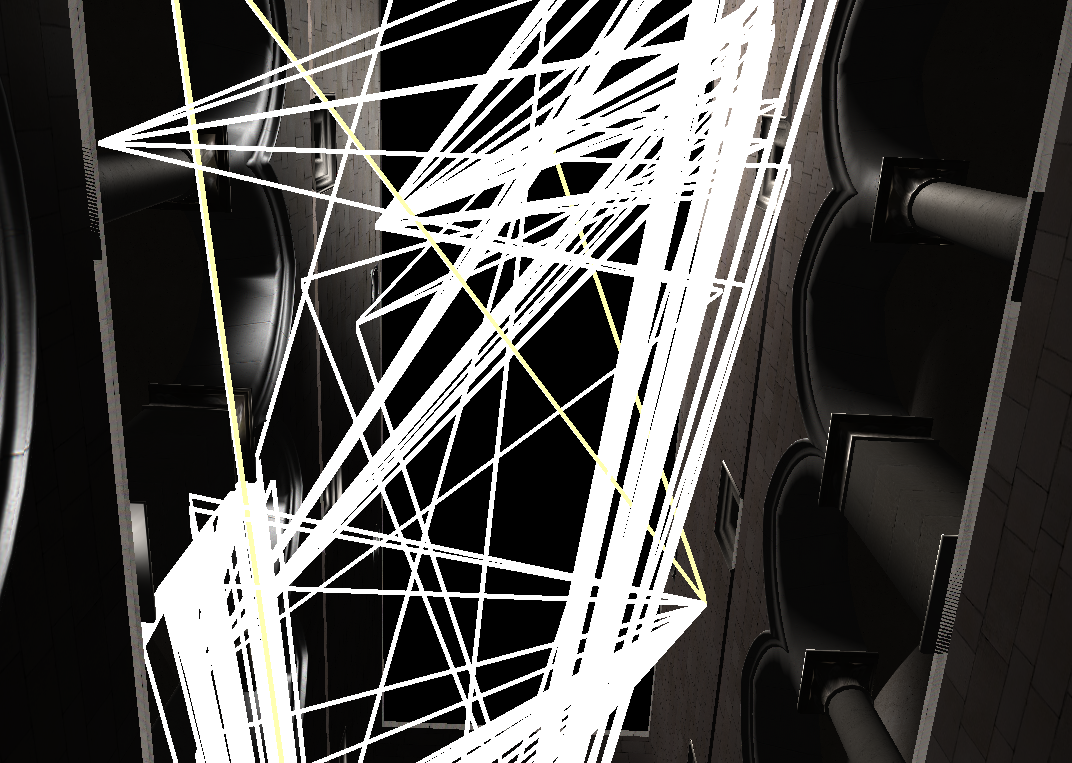
\includegraphics[width=0.5\textwidth]{paths.png}
    \caption{A large mass of generated light paths.}
    %\label{fig:mass}
\end{figure}

\begin{figure}[h]
    \centering
    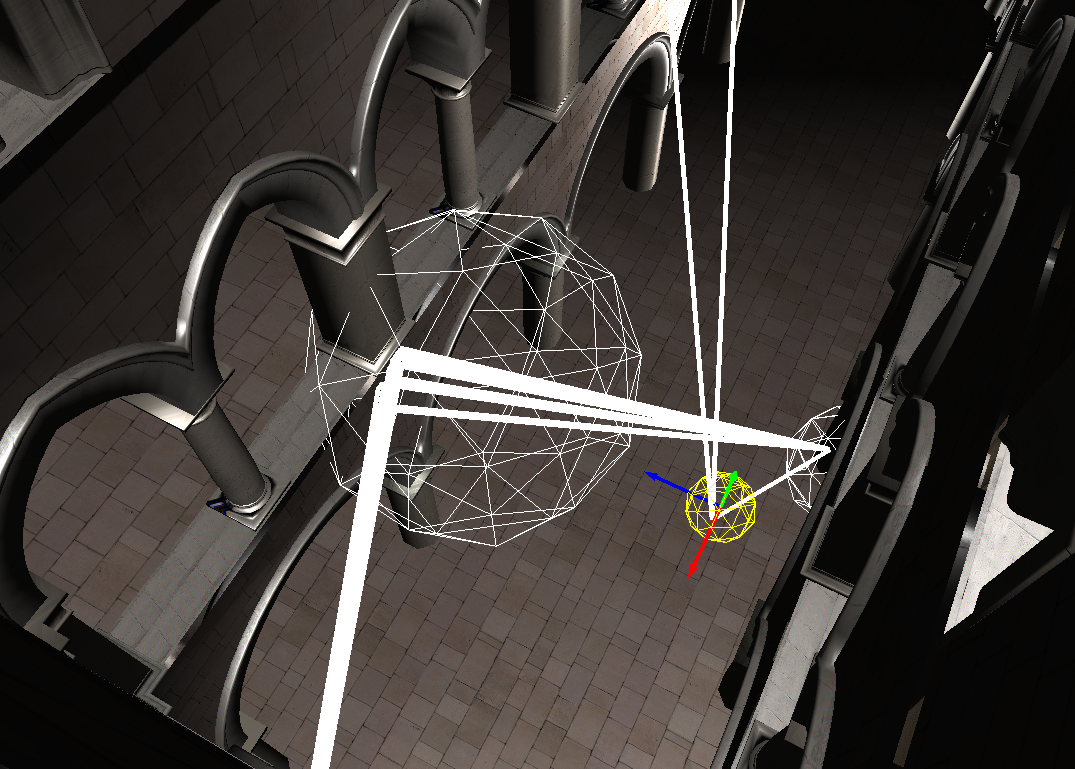
\includegraphics[width=0.5\textwidth]{selection.png}
    \caption{Path selection.}
    %\label{fig:mass}
\end{figure}

\begin{figure}[h]
    \centering
    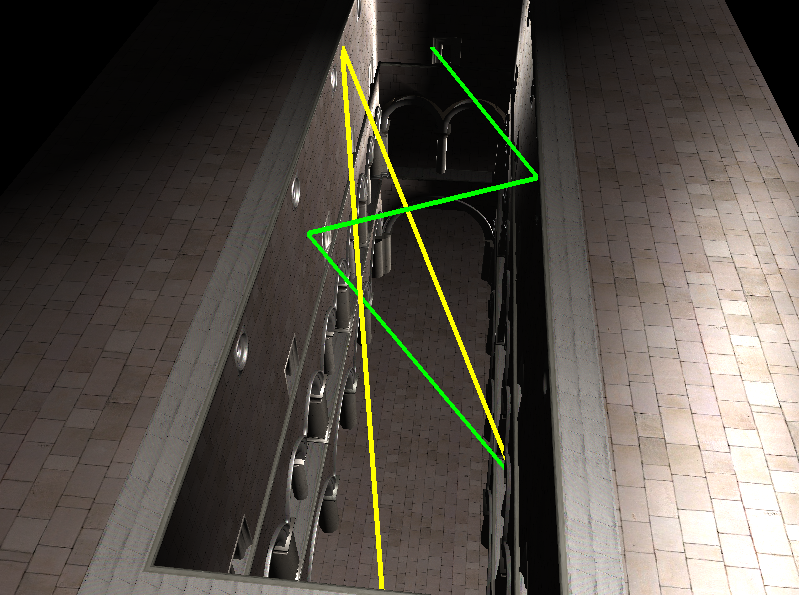
\includegraphics[width=0.5\textwidth]{single.png}
    \caption{Mutating a single path.}
    %\label{fig:mass}
\end{figure}

\begin{figure}[h]
    \centering
    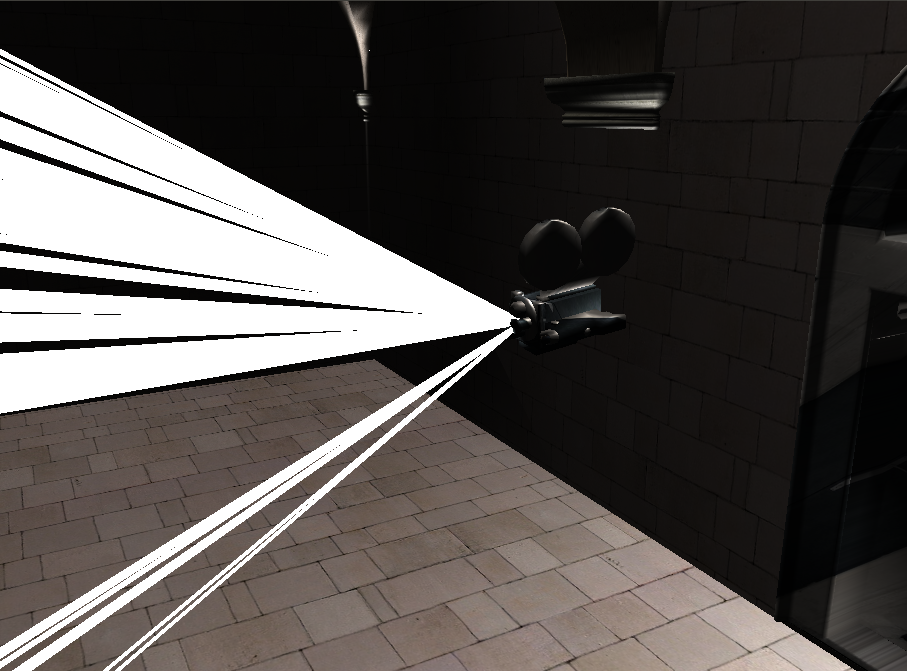
\includegraphics[width=0.5\textwidth]{camera.png}
    \caption{Virtual camera.}
    %\label{fig:mass}
\end{figure}

The program functions as expected. Yet, if we were to pinpoint it's biggest weakness, it would be in filtering of \texttt{inputPaths} when using selectors. Since we have to check every path vertex, this can be very slow with a massive amount of incoming data. Furthermore, because of the way MLT works, the light paths generated in a certain time period tend to be centered around a single scene region, and if we need to generate paths from a different one, it may take quite some time for the algorithm to get there. This problem would occur in the same way if we visualised ``live'', directly from the path tracer. In fact, it would be even more severe, because path mutations can take longer the a simple file parsing. 